% Created 2020-05-09 Sat 14:56
% Intended LaTeX compiler: pdflatex
\documentclass{article}
\usepackage[utf8]{inputenc}
\usepackage[T1]{fontenc}
\usepackage{graphicx}
\usepackage{grffile}
\usepackage{longtable}
\usepackage{wrapfig}
\usepackage{rotating}
\usepackage[normalem]{ulem}
\usepackage{amsmath}
\usepackage{textcomp}
\usepackage{amssymb}
\usepackage{capt-of}
\usepackage{hyperref}
\usepackage{algorithm2e}
\SetKw{KwInParallel}{in parallel}
\SetKw{KwThread}{thread}
\SetKw{KwAnd}{and}
\SetKw{KwExists}{exists}
\SetKwRepeat{Do}{do}{while}
\usepackage{float}
\author{Hanzhao Yu, Tonglin Chen\thanks{yuxx0839@umn.edu, chen5202@umn.edu}}
\date{\today}
\title{GPU Based Floor-planning Using Particle Swarm Optimization}
\hypersetup{
 pdfauthor={Hanzhao Yu, Tonglin Chen},
 pdftitle={GPU Based Floor-planning Using Particle Swarm Optimization},
 pdfkeywords={},
 pdfsubject={},
 pdfcreator={Emacs 26.3 (Org mode 9.1.9)}, 
 pdflang={English}}
\begin{document}

\maketitle
\begin{abstract}
This report summarizes our work for the final project of EE5302. We
implemented the sequence pair floorplanning algorithm using particle
swarm optimization on both standard multithreading C++ and CUDA. We tried
different velocity definition and compared the results. We found that 
CUDA on GPU provides an average of 3x of speed-up on large circuit 
comparing to multithreading C++ implementation.
\end{abstract}
\section{Introduction}
\label{sec:orgb5f1c7b}
The Floor-planning problem is a very important yet NP-Hard problem in the VLSI automation field. The input of this problem is a set of given circuit modules and their connections, as well as shapes. The general goal of floor-planning is to find a layout of the modules that minimize the total area and wire-length, as well as fit the overall shape requirement. Additional constraints for floor-planning could be fixed position of a certain block, fixed relative position of couple blocks, desired die area or aspect ratio, etc.  NP-hard problems like Floor-planning exists widely in the VLSI automation area. In order to solve these time-consuming but important problems, people will usually use heuristic algorithms in order to find a relatively good solution. The particle swarm optimization(PSO) is one of these nature-inspired, meta-heuristic algorithms. However, even heuristic algorithms like PSO have provided us an opportunity of solving NP-hard problems in a faster way. Sometime when the circuit is huge. It still takes a long time to finish all the iterations and reach a final result.
Recently, GPUs are widely used in many fields which requires massive parallel computation, such as machine learning and data analysis, thanks to the structure of GPU. There are multiple stream processors in GPU, each scheduling multiple threads at the same time. A lot of traditional algorithms have proved to be very efficient and could reach several times or even hundreds of times of speed improvement running on GPU when researchers have re-write the program properly. 
In this project, we first write a traditional PSO algorithm solving Floor-planning problems and then re-write the algorithm to run it on a NVidia GTX 1080 GPU trying to fully utilize the massive computation power GPU could provide and we have seen 3X in computation speed when running the program on GPU compared to the multi-threaded CPU implementation testing from Intel i7-7700. Along the way, we have also proposed a modified velocity representation used in the PSO algorithm for Sequence Pair, specifically dealing with permutation-based discrete searching space, adapted from previous works.
This project is done by two students. In this project,  Hanzhao focused on CPU implementation and Tonglin focused on GPU implementation. When it comes to optimization of the algorithm itself, we usually discuss it together.
\section{Background}
\label{sec:org1be7457}
\subsection{PSO Algorithm}
\label{sec:org448743e}
The Particle Swarm Algorithm is a nature-inspired, meta-heuristic algorithm. Originally proposed by Kennedy and Eberhart~\cite{PSO}. It was first inspired by and was trying to simulate social behavior. The key idea is that in a population, the movement of each individual is affected by its own history and the leader in this population. We could easily find that this is an oversimplified version of social behavior. More specifically, when this algorithm is used in optimization, it follows the steps shown in Figure~\ref{fig:PSO}.
\begin{figure}[H]
\centering
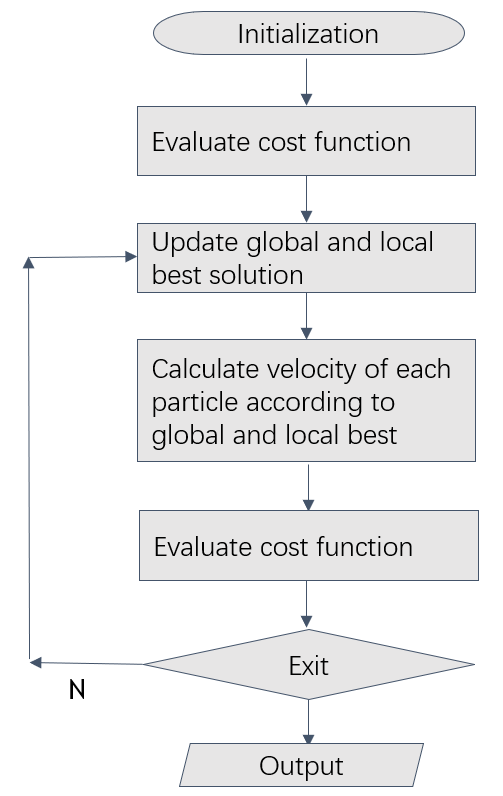
\includegraphics[width=0.4\linewidth]{PSO.PNG}
\caption{Flow chart of the Particle Swarm Optimization algorithm}
\label{fig:PSO}
\end{figure}
At the initialization step, a specific number of particles will be fist initialized. Each particle will be given an random initial solution. After that, the cost function will be evaluated for the first time and local best, global best solution is updated. Then, each particle will move according to the global best (the best solution among all the particles) and local best (the best solution this particle have ever reached) solutions. The position is updated and the cost will be evaluate again. We will then check if the exit condition is met, if not, we will go back and perform another iteration.
\subsection{Sequence Pair}
\label{sec:orga976d89}
The sequence pair representation~\cite{SeqPair} is first introduced by H. Murata, K. Fujiyoshi, S. Nakatake, and Y. Kajitani. In a rectangle based floor-planning problem. We could use two sequences (positive sequence and negative sequence respectively) represent one unique floor planning solution. By using sequence pair representation, we could ignore the complexity of actually placing the blocks. Instead, we can work on the pair of sequenced directly. After obtaining the positive sequence and the negative sequence, we will then need to build the constraint graph, called HCG (Horizontal Constraint Graph) and VCG (Vertical Constraint Graph) respectively based on the position of each block in the positive and negative sequence. And after that, a longest path algorithm will be executed to obtain the coordinate of each block, and this is one floor-planning solution.
\subsection{Other Heuristic Algorithms}
\label{sec:org045b8dd}
There are other nature-inspired, meta-heuristic algorithms like PSO.

Simulated annealing~\cite{5571036} is inspired by the annealing process that happened in nature. At the beginning of the process, crazy moves are allowed even if it increases the cost by a great amount, but as time moves on (the temperature decreases), the algorithm will become pickier and pickier in terms of the move until only the move will reduce the cost will be accepted. We have used this algorithm in VLSI automation 1, it has good result but the drawback is the very long running time. Which makes it not the best choice when the circuit is big.

The genetic algorithm~\cite{Shanavas_Gnanamurthy_2014} is inspired by evolution theory and in this paper, the author combines the genetic algorithm and simulated annealing algorithm to solve the NP-hard problem we discussed in the introduction. In the Genetic algorithm, operators like selection, crossover, and mutation will be performed on the population. And finally, over generations of evolution, the best cost will be improved over time and the best solution will then be selected as the final solution.

Cuckoo Search~\cite{5393690} is inspired by the behavior of a kind of bird called cuckoo, which has an aggressive reproduction strategy. Cuckoo will dump their egg in some other bird's nest. The risk exists when the bird will realize that there is an alien egg and take actions like finding a new nest or discard the alien egg. The Lévy Flights~\cite{5393690} is inspired by flight behavior such as fruit flies. They will use a series of sudden 90 degree turns until they find the final destination. And these two behavior has been implemented and mimicked in the optimization problem.

Ant Colony Optimization Approach~\cite{Arora2013CIRCUITPI} is inspired by the behavior of ants. In this algorithm, the searching agent(ant) will move through the search space to find the best solution. In the real world, and will lay down pheromones direction other ants while exploring the space. The search agent will also record their position and the solution quality. And in the later iterations, the search agent(ant) will focus more on the better solutions.

\section{Implementation Details}
\label{sec:orgb36a7e8}
In the project we implemented the algorithm on CUDA~\cite{cuda}, with the standard CUDA library and the cuRAND library. We also implemented a multi-threading CPU version in standard C++ as well, as the reference implementation. The reference implementation is simply one thread computing the results of certain particles. Since the computing results do not depend on the results from other particles except the global best update, it could be easily parallelized on CPU in each step updating all the particles at the same time. 
\subsection{Search Space and Velocity Update}
\label{sec:org8c66f6c}
As the original PSO algorithm is targeting at a continuous search space, we need alternative description or definition of the search space and velocity since our search space is two permutations of sequences. We found that the search space of Travel-Salesman Problem is also a permutation of sequence, therefore we tried to adapt some of the existing definitions from previous works.

The first definition of search space and velocity was adapted from~\cite{Clerc2004}. We first define a notation for the current \textit{sequence}, which is also the \textit{search space} in PSO, as \(X\). We define \(S=(a,b)\) as an operation to swap the \(a\)th element and \(b\)th element in the sequence. Therefore, the \textit{velocity} in PSO could be defined as a sequence of swap operations:
$$V = {S_1,S_2,S_3,S_4,...} $$
We define the \textit{add} operation  between two velocity \(V_A + V_B\) as to append all the swap operations in $V_B$ to $V_A$. Note the operation is not interchangeable. We define the operator $\oplus$ between a location and velocity \(X_A \oplus V_B\) as to apply the swap operations in $V_B$ to $X_A$. The difference between two \textit{location} $X_A-X_B$ is defined as the velocity to transform $X_B$ to $X_A$. Finally, the scalar multiplication of \textit{velocity} $\alpha V_A$, where $\alpha$ is between $[0,1]$ is defined as the \textit{velocity} containing the first $\lceil\alpha\operatorname{len}(V_A)\rceil$ swap operations in $V_A$.
Therefore the \textit{velocity} and \textit{location} for $k+1$th iteration and $i$th particle becomes:
\begin{equation}
    \begin{cases}
        \begin{split}
        V_i(k+1) &= \alpha V_i(k)+\beta [X_{lbest}-X_i(k)]+\gamma [X_{gbest}-X_i(k)]\\
        X_i(k+1) &= X_i(k)\oplus V_i(k+1)
        \end{split}
    \end{cases}
\end{equation}
Note that we could find the sequence of swap operations that transform a permutation in another in $n$ steps. The algorithm is described as followed:

\begin{algorithm}[H]
 \KwData{Source Permutation $S$, Target Permutation $T$, number of elements $n$}
 \KwResult{Swap Sequence $SS$}
 \For{$i\gets0$ \KwTo$n-1$}{
    $j\gets$ index of $T(i)$ in $S$\;
    swap $S(i)$ and $S(j)$\;
    $SS.\operatorname{insert}([i,j])$\;
 }
 \caption{Finding the swap sequence}
\end{algorithm}
Note the algorithm is sequential since for each step the data depend on previous steps. Note that the complexity is $O(n^2)$ sequential time, or $O(n)$ in parallel, assuming we have $n$ threads to perform algorithm.

The second definition was adapted from~\cite{1382191}. The search space here, is instead, the original PSO search space, which is a $n$-dimension vector of real number. We could map the vector to a permutation by sorting the vector, and assigning the sorted index to location of the element originally placed to get a permutation. The velocity then is also a $n$-dimension vector. In practice we would like to limit the search space. This could be done by setting boundary, and wrap the number back if it is out of bound.

The third definition was adapted from~\cite{1259748}. In this definition, we use the swap operator defined as the same with the first definition, but the definition of scalar multiplication with \textit{velocity} $\alpha V_A$ is modified. it is now defined as each operator in swap sequence will have a probability of $\alpha$ to take place, instead of length truncation. Also, we drop the term to keep previous velocity, as it would be hard 
to preserve all previous history. Instead, we add some random swap in the end so that the algorithm does not end at local minimum, usually 1\% of the number of elements. The updated search space could be defined in equation~\ref{eqn:vel3}.

\begin{equation}
\label{eqn:vel3}
    \begin{cases}
        \begin{split}
        V_i(k+1) &= \alpha [X_{lbest}-X_i(k)]+\beta [X_{gbest}-X_i(k)]+\operatorname{RandomSwap}\\
        X_i(k+1) &= X_i(k)\oplus V_i(k+1)
        \end{split}
    \end{cases}
\end{equation}

\subsection{CUDA Implementation}
\label{sec:orgcb68fbc}
In our implementation, each thread block represents one particle, and each thread in the block represent a module. In this way, some operation such as finding the location of an element in sequence (given the fact that is unique and exists, which is always the case in
our algorithm) could be executed in constant time in parallel.

In order to improve memory access proficiency, most intermediate results are stored in shared memory or registers, with the exception of HCG and VCG graphs in global memory, as they usually do not fit in the space of shared memory. These graphs are stored in adjacent matrix format.

Parallelization of HCG and VCG generation are pretty trivial, as each thread execute on its own given the order of its element in the sequence. The time complexity is $O(n)$ in parallel. Meanwhile, applying swap operators on sequences is complete sequential, since the order of swap operations would affect the final result, so we use one thread to perform the swapping operation. The time complexity is also $O(n)$.

We mainly focus on describing how we performed random swapping and topological sorting in parallel here.
\subsubsection{Random Swapping}
\label{sec:orgecc4c08}
Random swapping is useful to generate the initial sequence pair for each particle. The algorithm is perform swap in reduction manner shown in Figure~\ref{fig:swap}

\begin{figure}[htb]
\centering
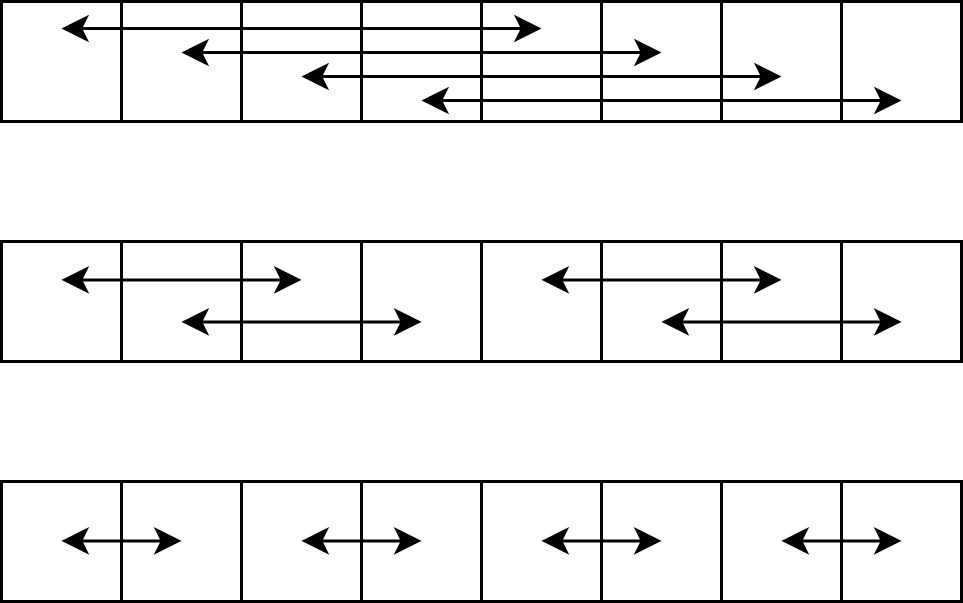
\includegraphics[width=0.5\linewidth]{Swap.PNG}
\caption{Example random swapping on 8 elements}
\label{fig:swap}
\end{figure}

Note that there is a problem in the algorithm. Assuming $n$ elements, the algorithm produces $\frac{n}{2}\log_2(\frac{n}{2})$ random swaps, so the size of result space would be at most $\frac{n}{2}^\frac{n}{2}$, which is far smaller than than the theoretical value $n!$, given the fact:
$$\lim_{n\to+\infty}\frac{\frac{n}{2}^\frac{n}{2}}{\Gamma(n)}=0$$
However, since the pseudo-random generator used today are not capable for generating all possible permutation for large enough circuit from our algorithm, let alone all possible permutations\footnote{For example, the number of possible permutation of a 100-module circuit for one sequence is $100!\approx2^{525}$, which is already larger than the possible variation of random seed. In cuRAND, the random seed used is a number with type \texttt{unsigned long long}, which is 64-bit by implementation~\cite{cuda}. Modern cryptography random number generator uses seed with length of 128-bit or 256-bit, which is still not enough for the purpose.}, we believe the implementation is fine in the use case. 
In general, we do not find it generating undesired bias than the CPU version in actual implementation.

\subsubsection{Parallel Topological Sort}
\label{sec:org9afab51}
To obtain the coordinate of each module, we would have to visit all the parents of this module to obtain the longest path to the current module in the constraint graph. Algorithm~\ref{alg:par_topo} is a parallel version of the classic Kahn's algorithm~\cite{KAHN10.1145/368996.369025} to topological sort a graph.

\begin{algorithm}[H]
 \KwData{Vertices $V$, Edges $E$}
 \KwResult{Vector Longest Path $LP$}
 $n\gets |V|$\;
 Queue $Q\gets \{\}$ \;
 Vector AddedToQ $\gets \{\}$\;
 Vector Income $\gets \{\}$\;
 \For{\KwThread $i\gets 0$ \KwTo$n-1$ \KwInParallel}{
    AddedToQ$[i] \gets$ false\;
    Income$[i] \gets$ number of incoming edges of $V[i]$\;
 }
 \Repeat{$Q$ is not empty} {
     \For{\KwThread $i\gets 0$ \KwTo$n-1$ \KwInParallel}{
        \If{Income$[i]==0$ \KwAnd AddedToQ$[i] ==$ false} {
              $Q$.atomicInsert(i)\;
              AddedToQ$[i] \gets$ true\;
        }
     }
     $j\gets$ $Q$.pop()\;
     Vector Path $\gets \{\}$\;
     \For{\KwThread $i\gets 0$ \KwTo$n-1$ \KwInParallel}{
        \If{$E(j\to i)$ \KwExists} {
            Income$[i]\gets$ Income$[i]-1$\;
        }
        \If{$E(i\to j)$ \KwExists} {
            Path$[i]\gets$ LP$[i]+E(i\to j)$\;
        }
        LP$[j]\gets$ max(Path$[0$ \KwTo $n-1]$)
     }
 }
 \caption{Finding the longest path using topological sort}
 \label{alg:par_topo}
\end{algorithm}

Note that we could build the Income vector simultaneously when we build the constraint graph. The time complexity for this algorithm in parallel, assuming we have $|V|$ threads, is $|V|\log|V|$, since there will be $|V|$ iterations, and each step in iteration could be done in constant time, except the \textbf{max} operation would require $O(\log(|V|))$ time to complete using parallel reduction. Note that this only works with Directed Acyclic Graph. If the graph does not satisfy the constraint, there will be vertices not visited by the algorithm.


\section{Results}
\label{sec:org75820d5}
In this section, we will present the result and analysis based on our test runs using the CPU multi-thread code and GPU multi-thread code. The CPU result is based on i7-7700, which has 4 core 8 threads in total. The GPU result is based on GTX 1080, which has 2560 CUDA cores in total.

The first result is about final cost VS population size shown in Figure~\ref{fig:FVP}.
\begin{figure}[H]
\centering
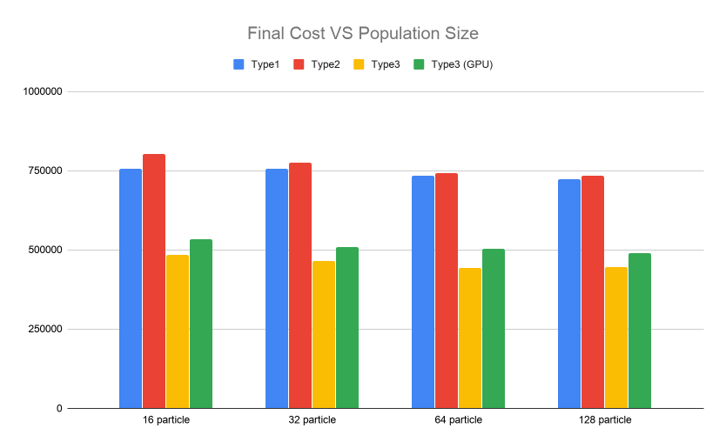
\includegraphics[width=1\linewidth]{CostVSPopulation.png}
\caption{Final Cost VS Population Size}
\label{fig:FVP}
\end{figure}

From figure~\ref{fig:FVP}, we could find that the population size has a limited effect on the final solution quality. In this particular example, the final solution result is improved slightly when we increase the population size from 16 to 32 and from 32 to 64. However, the improvement is negligible when we further improve the population size from 64 to 128. From figure~\ref{fig:FVP} specifically, we could draw the conclusion that 64 particles will give us the best result quality without doing meaningless work of supporting a large population.

We could also find that the type1 and type2 velocity representation will always have a worse result compared with type3. This result is consistent with other test runs and we will discuss them later.

The second result is about program run-time VS population size shown in figure~\ref{fig:TVP}
\begin{figure}[H]
\centering
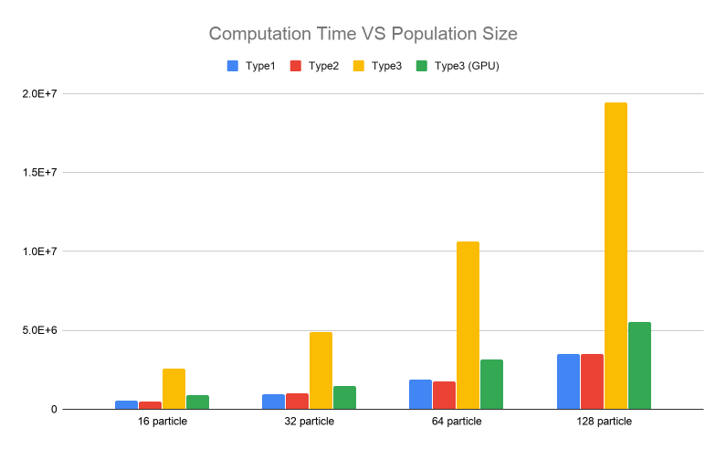
\includegraphics[width=1\linewidth]{TimeVSPopulation.png}
\caption{Run time VS Population Size}
\label{fig:TVP}
\end{figure}

From the above figure, it is obvious that the program run time has a linear relationship compared with the population size. This could be easily explained by the fact that we need to iterate through each particle and update the cost and location of each particle. More population simply means more calculation work. The type 1 and type 2 velocity representation running on CPU has a significantly shorter running time compared with type 3 velocity representation running on CPU. But form figure~\ref{fig:FVP}, they also have a worse final result. This is because the algorithm will easily be stuck in the local minimum and can not escape from it. And that is something we are trying to avoid in type3 representation as we were adding more randomness in the equation.

Also, we could find that by using GPU parallel computation, we have managed to reduce the calculation time by a factor of 3X or more.

The third result is about final cost VS circuit size shown in figure~\ref{fig:FVS}

\begin{figure}[H]
\centering
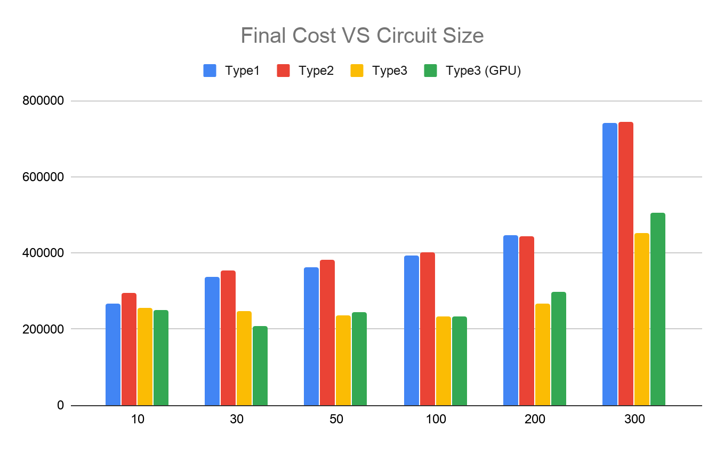
\includegraphics[width=1\linewidth]{CostVSsize.png}
\caption{Final cost VS Circuit Size}
\label{fig:FVS}
\end{figure}

The final cost of the floor-planning algorithm increases as the circuit size increases. But we can still find that the type 3 velocity representation has a clear advantage compared with type 1 and type 2, again, because for type 1 and type 2, the algorithm usually stuck in a local minimum and can't escape from it. Also, as the circuit size increases, the difference of type 3 representation over other representation also increases.  There is another problem in type 2 velocity policy, that points close to each other in search space does not essentially reflect to similar floor plan as result, so the local and global best might be meaningless with this policy.

The fourth result is about program run time VS circuit size shown in figure~\ref{fig:TVS}

\begin{figure}[H]
\centering
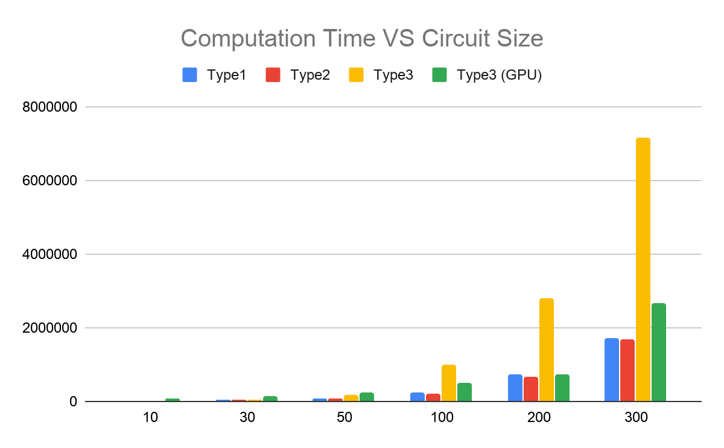
\includegraphics[width=1\linewidth]{TimeVSsize.png}
\caption{Run time VS Circuit Size}
\label{fig:TVS}
\end{figure}

From figure ~\ref{fig:TVS}, the first observation is that the run time of the program is an exponential function versus circuit size. This is the nature of NP optimization problems. Another observation is that we still see a 3X to 4X improvement when the circuit size is large, thanks to the enormous computation power GPU provide us. Compared with the huge advantage GPU has when the circuit is large, GPU performs worse than CPU when the circuit is small. This is because computation over-head, GPU need to communicate with the CPU even if the circuit size is small. We will also need to copy the required data back and forth from GPU to CPU. This amount of work exists no matter how big the circuit is.

\section{Conclusion and future work}
\label{sec:org2e01f19}
Overall, in this project, we have found that PSO\cite{PSO} algorithm is capable and could be used to solve a problem like sequence- pair-floor-planning which has a discrete searching space. To do that, we introduced three types of velocity representation. All of them are permutation-based discrete search space velocity. Among the three velocities, type 3 velocity representation has a clear advantage in terms of the result-quality. However, the drawback of type3 velocity representation is the significantly longer run time. To solve this problem, our solution is to use GPU. From the result we could find that GPU has a 3X improvement in terms of run time. It can obtain a much better result with a similar running time compared with type 1 and type 2 representation.

The next step of this project includes these possible directions:
\begin{itemize}
    \item Sparse Matrix could be used to represent the HCG and VCG, there are specific algorithms to store and transfer sparse matrix, which can save the memory bandwidth and improve the efficiency of communication between the CPU and GPU, and between the different threads within the GPU. Note that using this kind of representation, we could further parallel the process efficiently by executing the items added to the queue in the algorithm at the same time in parallel, but the incoming edge representation could be a little bit trickier.
    \item A better permutation-based search space update policy could be found. We have already seen the impact and importance of the velocity policy have on the final solution quality. A better policy could potentially offer a better result and a shorter running time.
    \item So far the largest circuit we have tested on contains 300 blocks. And this could not demonstrate clearly how this algorithm scales as the circuit size increases. More tests on a larger circuit will be helpful.
    \item Detect GPU bottleneck and further improve the computation speed. The performance of GPU computation is limited by multiple different aspects. Such as memory bandwidth, local memory resources, and bandwidth between CPU/GPU, and so on. If we could detect which is the limiting factor for the current program and modify the algorithm accordingly, we will be able to further improve the GPU performance. 
\end{itemize}

\bibliographystyle{ieeetr}
\bibliography{ref}
\end{document}